\lfoot{Autor: Tobias Perny}
\subsection{Car-PC}
\label{subsec:carpc}

Da nicht alle notwendigen Daten direkt aus der OBDII Schnittstelle ausgelesen werden können, wird ein PC gebaut, welcher in die Mittelkonsole eines KFZ integriert werden kann.
Dieser PC soll einen Single-Board PC und Sensoren enthalten, welche eben diese Daten über eine Bluetooth Verbindung an ein Smartphone senden kann.

\subsubsection{Single-Board-Computer}
Eine wichtige Komponente des Car-PC's ist der Single-Board-Computer \textit{Einplatinencomputer oder SBC}, alle anderen Komponenten hängen von diesem ab.

\textbf{Ziele\newline}
Für die Auswahl der Hardware für den Car-PC wurden folgende Kriterien in Betracht gezogen:
\begin{itemize}
\item Der PC muss Sensoren direkt ansprechen können und dafür notwendige Schnittstellen anbieten:
\begin{itemize}
\item Internet
\item Bluetooth
\end{itemize}
\item  Der PC muss in die Mittelkonsole eines KFZ eingebaut werden können. Dadurch ergeben sich maximale Maße: 
\begin{itemize}
\item Breite 6.5 cm
\item Länge 18 cm
\item Tiefe 5 cm
\end{itemize}
\item Er muss Ausreichend Speicher damit alle gesammelten Daten einer Autofahrt in einer Datenbank gespeichert werden können.
\end{itemize}


\textbf{Realisierung\newline}
\newline
Lösungsansatz
Es wurden grundsätzlich zwei Lösungsansätze in Betracht gezogen.

\begin{itemize}
\item Ansatz 1: Tinkerforge RED Brick
Der RED Brick von Tinkerforge ist ein Single-Board PC mit vielen Funktionen.
Mithilfe des RED Bricks ist es möglich andere Bricklets der Firma über eine proprietäre schnittstelle anzusteuern und somit Daten auszulesen.
Mit dieser Lösung ist es also möglich ein „Temperatur“ und ein „Beschleunigungs-Bricklet“ an den RED Brick anzuschließen und somit alle notwendigen Daten der Fahrt speichern.
Er ünterstützt außerdem ein breites Spektrum an Programmiersprachen.
[Quelle: \url{https://www.tinkerforge.com/de/shop/bricks/red-brick.html}]

\item Ansatz 2: Raspberry PI 2 Modell B
Der Raspberry PI 2B ist das Modell der jüngsten Generation des Raspberry PI. Er besitzt einen 900MHz quad-core Prozessor und 1 Gigabyte RAM. Darüber hinaus hat er 4 USB Ports und einen HDMI Anschluss. Durch seine 40 GPIO pins ist es möglich über i²C jeden damit kompatiblen Sensor anzuschließen und somit die benötigten Daten der Fahrt zu speichern.
Der Raspberry PI 2B unterstützt weniger Programmiersprachen als der RED Brick von Tinkerforge.
\end{itemize}

\textbf{Umsetzung\newline}
\newline
Es wurde der Raspberry PI zum umsetzen des Projektes gewählt aufgrund folgender Tatsachen:
Modularität:
Wir sind dank der GPIO Pins des Raspberry PI nicht auf andere Geräte derselben Firma angewiesen und können jeden Sensor verwenden, der mit diesen GPIO Pins kommunizieren kann.
Peripherie:
Der Raspberry PI 2B besitzt 4 USB Ports. Mithilfe dieser Ports ist es möglich Bluetooth-Adapter und WLAN-Adapter, anzuschließen.
\newpage
\textbf{Wirtschaftlichkeit\newline}
\newline
Der Raspberry PI 2B kostet EUR 34,99 bei einem offiziellen Anbieter der Firma.
\url{https://www.element14.com/community/community/raspberry-pi}
Der Preis des „RED Brick“ beträgt EUR 69,99 beim Anbieter direkt.
\url{https://www.tinkerforge.com/de/shop/bricks.html}
Das bedeutet der Raspberry PI 2B ist um fast die Häfte günstiger als der RED Brick, und aufgrund der
Modularität des Raspberry PI können auch billigere Sensoren verwendet werden als beim tinkerforge
RED Brick.

\subsubsection{Verbaute Sensoren}
Nicht alle Daten die wir für unsere Android App benötigen, werden von der OBDII Schnittstelle
zurückgegeben. Um diese zu erhalten müssen zusätzlich zum SBC (Single-Board-Computer) zwei Sensoren im fertig Car-PC enthalten sein.
\nextline
\textbf{Ziele\newline}
\newline
Die Android App soll in der Lage sein die Beschleunigung in 3 Achsen darzustellen, und dem Benutzer
die Innenraumtemperatur des Wagens mitzuteilen.
Hierfür werden ein Beschleunigungssensor und ein Temperatursensor mit dem SBC kommunizieren
um die gewünschten Werte zu erhalten.
\nextline
\textbf{Realisierung\newline}
\newline
Da ein Raspberry PI 2B als Hauptplatine gewählt wurde, wissen wir welche Sensoren für dieses Projekt in Frage gekommen sind.
\nextline
\textbf{Umsetzung\newline}
\newline
Es wurden I2C fähige Sensoren zur Umsetzung des Projektes gewählt, weil der Raspberry Pi dank seiner gpio Pins in der Lage ist mit I2C fähigen Sensoren zu kommunizieren. Da dieser Bus sehr einfach zu konfigurieren ist und diese Art von Sensoren somit sehr leicht zu Handhaben sind.
Bei dieser Art von Sensoren gibt es 2 Pins auf welche geachtet werden müssen. Diese haben die Bezeichnungen SDA und SCL. Sobald diese Pins mit denen des Raspberry PI verbunden sind bekommt der Sensor eine Slave Adresse zugewiesen. Mithilfe dieser kann man die Daten auslesen.
\begin{figure}[!htb]\centering
	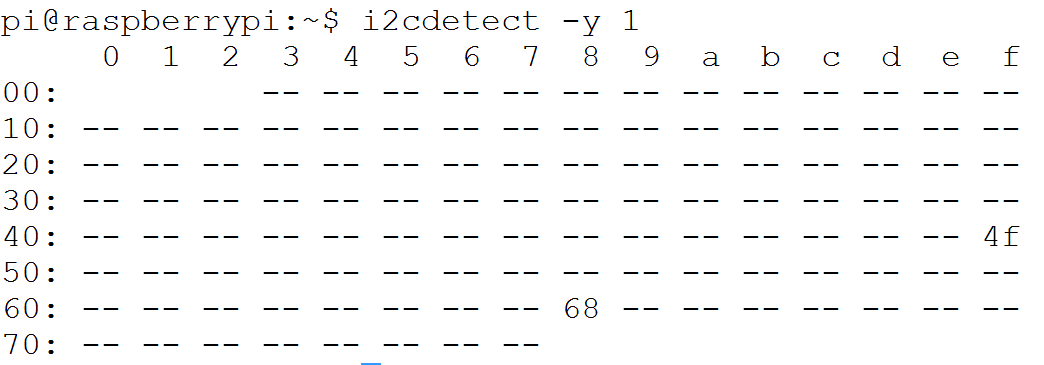
\includegraphics[width=0.5\textwidth]{images/sensorendetect}
	\caption{Beispielhafte Ausgabe von am I2C-Bus erkannten Slave-Devices mit den Adressen 4f und 68}\label{Fig:imgSensorDetect}
\end{figure}
\newpage
\textbf{Wirtschaftlichkeit\newline}
\newline
Konkret wurden ein GY521 Beschleunnigungssensor und ein DS1621 Temperatursensor im Car-PC verbaut. Diese beiden sind für insgesamt etwa EUR 15 (Stand 04 2016 [amazonquelle]) Online erhältlich.

\begin{figure}[!htb]\centering
   \begin{minipage}{0.49\textwidth}
     \frame{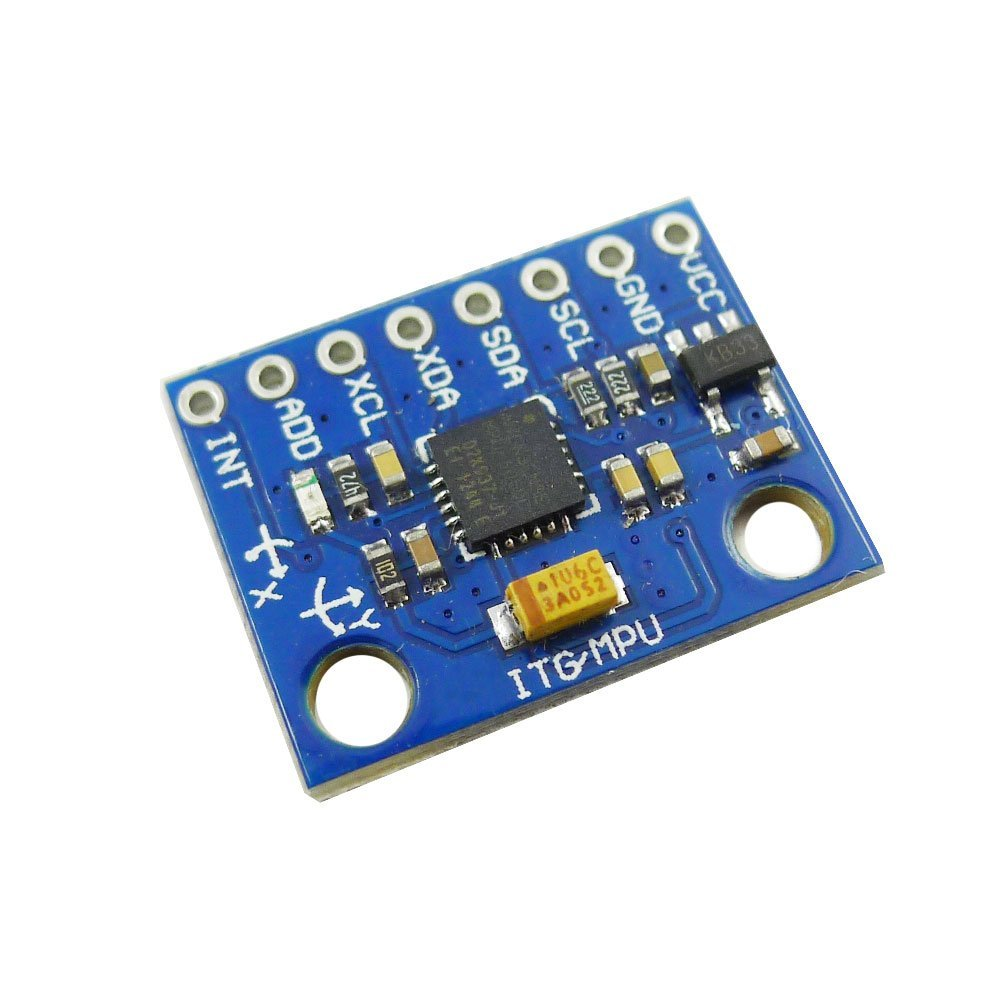
\includegraphics[width=\linewidth]{images/gy521}}
     \caption{Ein GY521 Beschleunigungssensor \cite{PERT.CH3-carpc.gy521}}\label{Fig:imgGY521}
   \end{minipage}
   \begin {minipage}{0.49\textwidth}
     \frame{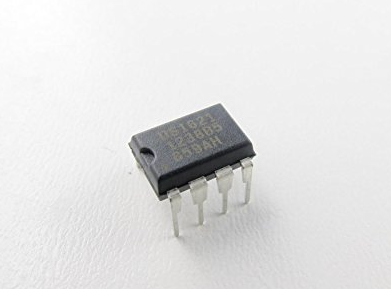
\includegraphics[width=\linewidth]{images/ds1621}}
     \caption{Ein DS1621 Temperatursensor \cite{PERT.CH3-carpc.ds1621}}\label{Fig:imgDS1621}
   \end{minipage}
\end{figure}




\clearpage % DO NOT REMOVE